\documentclass{beamer}
\usepackage{lmodern}
\usepackage[export]{adjustbox}
\usepackage{graphicx}
\usepackage{tikz}
\usepackage{hyperref}
\usepackage{geometry}

\usetheme{Madrid}

\hypersetup{
    urlcolor=blue,
    }

\usepackage{smartdiagram}

\usesmartdiagramlibrary{additions} % required in the preamble
\usetikzlibrary{arrows} % required in the preamble

\smartdiagramset{
    uniform color list=orange!60!yellow for 5 items,
    circular final arrow disabled=true,
    circular distance=2.25cm,
    arrow tip=to,
    arrow line width=2pt,
    additions={
        additional item bottom color=orange!60!yellow,
        additional item border color=gray,
        additional item shadow=drop shadow,
        additional item offset=0.65cm,
        additional arrow line width=2pt,
        additional arrow tip=to,
        additional arrow color=orange!60!yellow,
}
}

\title{Generare MIDI folosind algoritmi genetici}
\author{Gheorghe Andrei}
\date{Septembrie, 2022}

\begin{document}
\begin{frame}
    \titlepage{}
\end{frame}

\begin{frame}
    \frametitle{Cuprins}
    \tableofcontents
\end{frame}

\section{Arhitectură}

\begin{frame}
    \begin{centering}
        \begin{beamercolorbox}[sep=12pt,center,rounded=true]{part title}
            \usebeamerfont{title}\insertsection\par
        \end{beamercolorbox}
    \end{centering}
\end{frame}

\begin{frame}{Arhitectură}
\begin{itemize}
    \item Aplicația este compusă dintr-un modul de python, un plugin audio, și o librărie care "leagă" primele două componente.
    \item Pe lângă acestea, proiectul folosește 4 librării externe: pybind11, JUCE, Boost, și foleys\_gui\_magic.
    \item Librăria comună folosește pybind11 pentru a permite interoperabilitate între plugin-ul scris în C++ și modulul de python.
    \item Astfel, aceasta definește 2 clase, utilizate atăt în implementarea modulului, cât și un API care abstractizează apelarea funcțiilor prin interpretatorul încorporat de pybind11.
    \item Componentele aplicației, cât și librăriile externe sunt construite și "împachetate" folosind CMake. 
\end{itemize}
\end{frame}

\begin{frame}
\begin{center}
    \begin{figure}
        \centering
        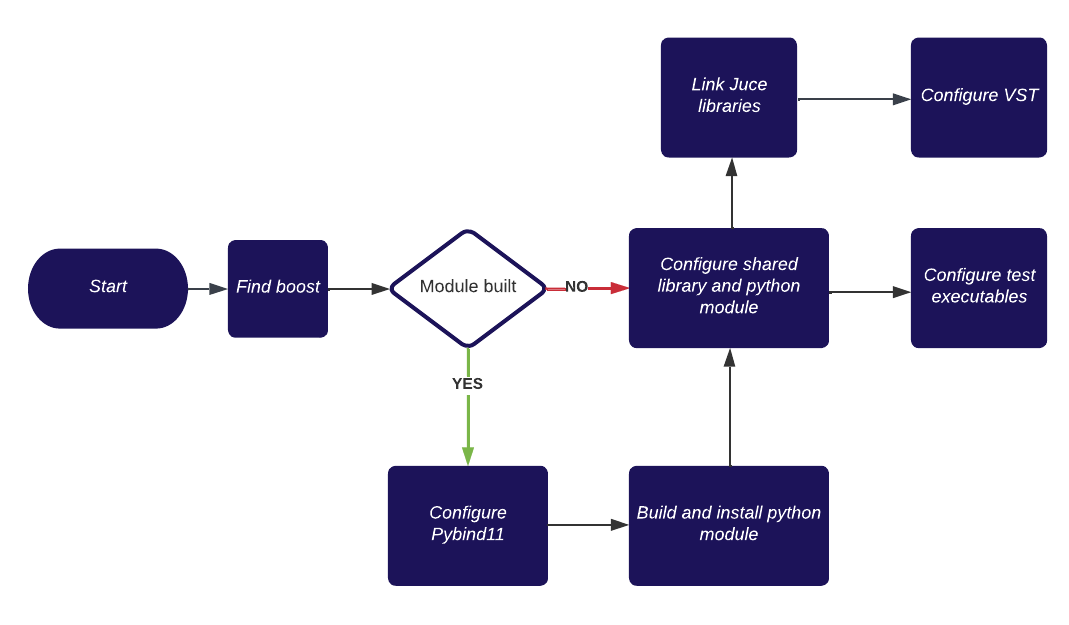
\includegraphics[scale=0.7]{Architecture.png}
    \end{figure}
\end{center}
\end{frame}

\section{Python module}
\begin{frame}
    \begin{centering}
        \begin{beamercolorbox}[sep=12pt,center,rounded=true]{part title}
            \usebeamerfont{title}\insertsection\par
        \end{beamercolorbox}
    \end{centering}
\end{frame}

\begin{frame}{Algoritm genetic}
\begin{itemize}
    \item Modulul de python implementează algoritmii genetici folosiți în cadrul aplicației. Acest lucru este realizat folosind framework-ul deap.
    \item Modulul conține două seturi de operatori genetici, unul pentru funcția "generate", și unul pentru funcțiile "continue" și "combine".
    \item Primul algoritm este un algoritm genetic multiobiectiv și folosește operatorul de selecție NSGA-II.
    \item Algoritmul evaluează fitness-ul unui individ în funcție de nivelul de sincopare, densitatea notelor, și rația notelor consonante.
    \item Nivelul de sincopare poate fi calculat folosind măsura WNBD sau Off-beatness.
    \item Pentru al doilea algoritm, fitness-ul unui individ este calculat folosind funcția NCD (Normalized Compression Distance).
\end{itemize}
\end{frame}

\begin{frame}
    \begin{figure}
        \centering
        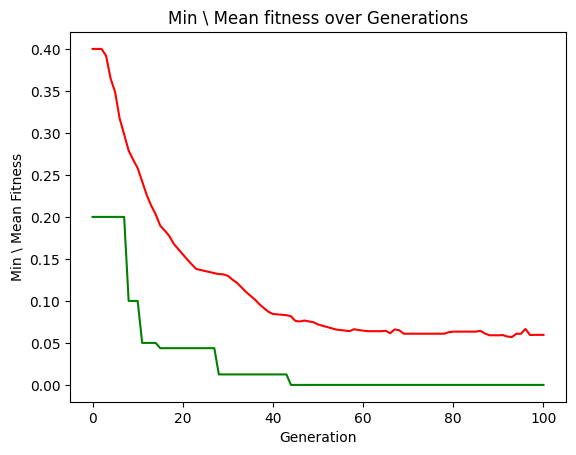
\includegraphics[scale=0.65]{genetic.png}
        \caption{Evoluția fitness-ului folosind măsura WNBD pentru sincopare}
    \end{figure}
\end{frame}

\begin{frame}
    \begin{figure}
        \centering
        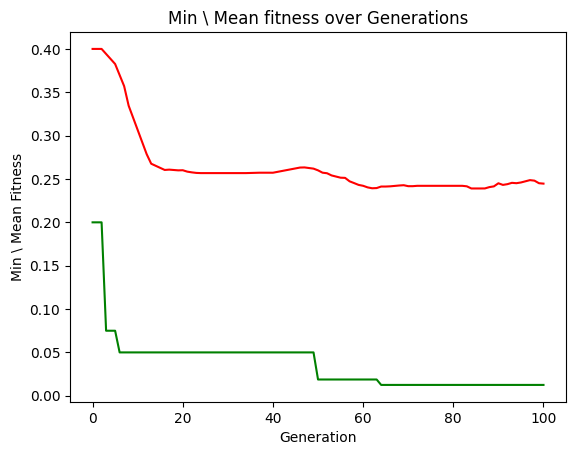
\includegraphics[scale=0.65]{genetic_WNBD.png}
        \caption{Evoluția fitness-ului folosind măsura Off-beatness pentru sincopare}
    \end{figure}
\end{frame}

\begin{frame}{Algoritm genetic}
\begin{itemize}
    \item Ambii algoritmi folosesc aceeași codificare a genelor și aceiași operatori de mutație și de recombinare.
    \item Secvențele muzicale sunt codificate sub forma unei liste formate din frecvența, velocitatea și durata rămăsa din nota redată în momentul fiecărui puls.
    \item Operatorul de recombinare folosit este încrucișarea cu un singur punct.
    \item Mutația poate să afecteze frecvența, velocitatea, sau durata unei note.
    \item Un wrapper este definit peste operatorii de mutație și încrucișare pentru a corecta durata rămasă din notă pentru fiecare puls după aplicarea acestora.
\end{itemize}
\end{frame}

\section{Audio plugin}
\begin{frame}
    \begin{centering}
        \begin{beamercolorbox}[sep=12pt,center,rounded=true]{part title}
            \usebeamerfont{title}\insertsection\par
        \end{beamercolorbox}
    \end{centering}
\end{frame}

\begin{frame}{Audio plugin}
    \begin{itemize}
        \item Plugin-ul audio este scris folosind framework-ul JUCE și librăriile foleys\_gui\_magic și Boost.
        \item Acesta este distribuit atât sub forma unei aplicații de sine stătătoare, cât și în format VST și AU, pentru a putea fi deschis într-un DAW.
        \item Interfața grafică a acestuia conține 3 elemente principale: un piano roll, un filetree, și un panou de configurare.
        \item Piano roll-ul este folosit pentru a vizualiza și modifica secvențele muzicale. O secvență este formată dintr-o listă de note.
        \item Notele sunt reprezentate într-o clasă care extinde forma de dreptunghi a framework-ului JUCE și încapsulează o notă definită în librăria comună.
    \end{itemize}
\end{frame}

\begin{frame}{Audio plugin}
    \begin{itemize}
        \item Filetree-ul poate parcurge directoarele sistemului intern de fișiere, poate salva fișiere în format MIDI, și poate încărca secvențe în piano roll.
        \item Pentru a salva fișiere este folosită funcția "write\_file" din cadrul modului de python.
        \item Pentru a încărca fișiere, aplicația folosește funcționalitățiile din librăria JUCE pentru a extrage și transforma mesajele de tipul "Note on" și "Note off" din fișier.
        \item Panoul de configurare conține 4 tab-uri, câte unul pentru fiecare dintre funcționalitățiile expuse de aplicație, și un buton de "run", comun tuturor celor 4 ferestre.
    \end{itemize}
\end{frame}

\section{Posibile dezvoltări ulterioare}
\begin{frame}
    \begin{centering}
        \begin{beamercolorbox}[sep=12pt,center,rounded=true]{part title}
            \usebeamerfont{title}\insertsection\par
        \end{beamercolorbox}
    \end{centering}
\end{frame}

\begin{frame}{Posibile dezvoltări ulterioare}
    \begin{itemize}
        \item În momentul de față funcțiile "generate" și "continue" nu funcționează corespunzător. Această problemă ar putea fi rezolvată prin schimbarea metodei de codificare a indiviziilor. 
        \item Comportamentul celor 2 funcții poate fi folosit însă pentru a crea o funcționalitate nouă, anume transformarea unei melodii într-o progresie de acorduri.
        \item Momentan, plugin-ul nu interacționează deloc cu DAW-ul în care este deschis; secvențele generate trebuie salvate într-un fișier și apoi încarcate în DAW.
        \item Plugin-ul ar putea trimite mesaje MIDI în loc să creeze fișiere. Acestea ar putea fi apoi recepționate direct în DAW.
    \end{itemize}
\end{frame}

\end{document}